\documentclass[a4paper]{article}

\usepackage{amsmath}
\usepackage{amssymb}
\usepackage{stellar}
\usepackage{parskip}
\usepackage{fullpage}
\usepackage{wrapfig}
\usepackage{tikz}

\usetikzlibrary{arrows}
\usetikzlibrary{decorations.pathreplacing}

\title{Fisica I}
\author{Paolo Bettelini}
\date{}

% libri
% Rosati

\begin{document}

\maketitle
\tableofcontents

\section{Introduzione}

\section{Vettori spostamento}

\begin{itemize}
    \item vettore spostamento: direzione, verso, lunghezza;
    \item somma di vettori;
    \item moltiplicazione con scalare reale \(\vec{a} + (-\vec{a}) = \vec{0}\);
    \item modulo di un vettore;
\end{itemize}

\sproposition{Proprietà distributiva del prodotto rispetto alla somma vettoriale}{
    \[\alpha(\vec{a} + \vec{b}) = \alpha\vec{a} + \alpha\vec{b}\]
}

\section{Sistemi di coordinate}

Il punto di origine è il posto in cui viene posizionato l'osservatore.
I sistemi di coordinate trattati sono esclusivamente cartesiani e con basi ortogonali.
L'oservatore ha i versori delle direzioni.

Si possono quindi individuare le componenti di un vettore lungo le sue direzioni, ossia
le proiezioni ortogonali del vettori lungo gli assi cartesiani.
Di conseguenza, le coordinate di un vettore hanno senso solamente rispetto ad una base.

\sdefinition{Prodotto scalare}{
    Il prodotto scalare fra due vettori risulta in un numero reale (in uno spazio euclideo \(\mathbb{R}^n\))
    \[
        \vec{a} \cdot \vec{b} \in \mathbb{R}
    \]
    Dato l'angolo \(\theta\) fra \(\vec{a}\) e \(\vec{b}\),
    \[
        \vec{a}\cdot \vec{b} = |\vec{a}| \cdot|\vec{b}| \cdot \cos\theta
    \]
}

Chiaramente il prodotto scalare è commutativo.

\sproposition{Proprietà distributiva del prodotto scalare rispetto alla somma}{
    \[
        \vec{c} \cdot (\vec{a} + \vec{b}) = c\vec{a} + c\vec{b}
    \]
}

\sproposition{Prodotto vettoriale con componenti}{
    TODO....
}

Da qui possiamo notare che il prodotto scalare ha lo stesso ridultato per ogni basta ortonormata.

% fai il prodotto fra c e a+b, e poi espandi la distributiva e semplifica i termini ortogonali.

\sdefinition{Prodotto vettoriale}{
    Il prodotto scalare fra due vettori risulta in un vettore (in uno spazio euclideo \(\mathbb{R}^n\))
    \[
        \vec{a} \wedge \vec{b} \in \mathbb{R}
    \]
    Dato l'angolo \(\theta\) fra \(\vec{a}\) e \(\vec{b}\),
    il risultato è un vettore con modulo
    \[
        |\vec{a} \wedge \vec{b}| = |a||b|\sin\theta
    \]
    e direzione normale al piano formato da \(\vec{a}\) e \(\vec{b}\).
    Convenzionalmente, il verso del vettore normale è scelto secondo 
    la regola della mano destra.
}

\sproposition{Proprietà del prodotto vettoriale}{
    \begin{enumerate}
        \item \(\vec{a} \wedge \vec{b} = - \vec{b} \wedge \vec{a}\);
        \item \((\gamma \vec{a}) \wedge \vec{b} = \gamma (\vec{a} \wedge \vec{b})\);
        \item \((\vec{a} + \vec{b}) \wedge \vec{c} = \vec{a} \wedge \vec{c} + \vec{b} \wedge \vec{c}\)
    \end{enumerate}
}

Consideriamo \(\vec{a}\) e \(\vec{b}\), allora
\begin{align*}
    \vec{a} &= a_x\hat{x} + a_y\hat{y} + a_y\hat{z} \\
    \vec{b} &= b_x\hat{x} + b_y\hat{y} + b_y\hat{z}
\end{align*}
Sapendo che
\begin{align*}
    \hat{x} \wedge \hat{y} &= \hat{z} \\ 
    \hat{x} \wedge \hat{z} &= -\hat{y} \\
    \hat{y} \wedge \hat{z} &= \hat{x} \\
\end{align*}
Possiamo eseguire il prodotto esplicitamente
\begin{align*}
    \vec{a} \wedge \vec{b} &= a_xb_y\hat{z} + a_xb_z(-\hat{y}) + a_yb_x(-\hat{z})
    + a_yb_z\hat{x} + a_zb_x\hat{y} + a_zb_y(-\hat{x}) \\
    &= \left[a_yb_z - a_zb_z\right] \hat{x} + \left[a_zb_x - a_xb_z\right]\hat{y}
    + \left[a_xb_y - a_yb_x\right] \hat{z}
\end{align*}

\pagebreak

\section{Cinematica}

La cinematica è la parte della meccanica che descrive il moto di un punto materiale.
Per descrivere il moto di un oggetto è necessario procurarsi un sistema di riferimento.
Sceglieremo quindi un'origine e una base ortonormata.

\sdefinition{Posizione}{
    La \textit{posizione} di un punto è rappresentata unicamente da un vettore \(\vec{r}(t)\),
    che mostra lo spostamento fra l'origine e la sua posizione \(P(t)\) in un determinato istante di tempo.
}

Se vogliamo considerare la posizione solo nella direzione \(x\)
possiamo calcoalre
\[
    \hat{x}(t) = \vec{x}\vec{r}(t)
\]
In generale
\[
    \vec{r}(t) = \hat{x}\vec{r}(t) + \hat{x}\vec{y}(t) + \hat{z}\vec{r}(t)
\]

La relazione fra due osservatori diversi è data da \(\vec{R} + \vec{r'}(t) = \vec{r}(t)\).

La velocità è quindi relativa a due posizioni \(P(t)\) e \(P(t + \Delta t)\).
Lo spostamento è \(\vec{r}(t + \Delta t) = \vec{r}(t) + \vec{s}(t)\).

\sdefinition{Velocità}{
    La \textit{velocità} di un punto rappresenta lo spostamento che il punto materiale
    percorre in un unità di tempo \(\vec{v}(t)\).
    Allora la velocità è definita come
    \[
        \vec{v}(t) = \lim_{\Delta t \to 0} \frac{\vec{s}}{\Delta t}
        = \lim_{\Delta t \to 0} \frac{\vec{r}(t+\Delta t) - \vec{r}(t)}{\Delta t}
        = \frac{d\vec{r}(t)}{dt}
    \]
}

Il vettore della velocità si orienta verso la tangente della curva (cioè nella direzione in cui si sta spostando).
Chiaramente la derivata può essere separata nelle componenti
\[
    \vec{v}(t)=v_x\hat{x} + v_y\hat{y} + v_z\hat{z}
\]
dove possiamo anche dire che
\[
    v_x(t) = \frac{dx(t)}{dt}
\]

\sdefinition{Accelerazione}{
    L'\textit{accelerazione} di un punto rappresenta il cambiamento istantaneo della velocità
    \[
        \vec{a}(t) = \lim_{\Delta t \to 0} \frac{\vec{v}(t + \Delta t) - \vec{v}(t)}{\Delta t}
    \]
}

\section{Leggi orarie}

\sproposition{Caduta da una altezza}{
    Il tempo di caduta di un oggetto da un altezza \(h\), soggetto a gravità costante \(g\)
    è cado da
    \[
        t_\text{caduta} = \sqrt{\frac{2h}{g}}
    \]
    con velocità
    \[
        -\sqrt{2gh}
    \]
}

\pagebreak

\section{Moto arbitrario}

Consideriamo un moto arbitrario \(\vec{r}(t)\). Questo vettore punta sempre alla posizione dell'oggetto.
La sua velocità \(\vec{v}(t) = \frac{d\vec{r}(t)}{dt}\) è un vettore sempre nella direzione della traiettoria.
Definiamo allora il versore tangente
\[
    \hat{T}(t) v(t) = \vec{v}(t)
\]
Abbiamo allora che
\[
    \vec{a}(t) = \frac{d}{dt} \left(v(t)\hat{T}(t)\right) = \frac{dv(t)}{dt}\hat{T}(t) + v(t)\frac{d\hat{T}(t)}{dt} = a_t(t)\hat{T}(t) + v(t)\frac{d\hat{T}(t)}{dt}
\]
La prima componente, \(\frac{dv(t)}{dt}\hat{T}\), è chiamamta \textit{accelerazione tangenziale}
mentre il secondo \textit{accelerazione centripeta} (entrambi sono perpendicolari fra di loro).

Per studiare il significato di tale termine, cominciamo partendo dall'identità \(\hat{T}(t) \cdot \hat{T}(t) = 1\).
Allora,
\begin{align*}
    \frac{d}{dt} \left( \hat{T}(t) \cdot \hat{T}(t) \right) &= 0 \\
    \frac{d\hat{T}(t)}{dt} \cdot \hat{T}(t) + \hat{T}(t)\frac{d\hat{T}(t)}{dt} &= 0 \\
    \hat{T}(t)\frac{d\hat{T}(t)}{dt} &= 0 
\end{align*}
Dall'analisi differenziale troviamo che
\[
    \left|\frac{\hat{T}(t)}{dt}\right| = \lim_{\Delta t \to 0} \frac{dl}{\Delta t}
\]
e l'arco di circonferenza
\[
    s = Rd\theta
\]
dove \(R\) è la lunghezza della retta fino al punto di rotazione (raggio di curvatura, ossia il raggio del cerchio osculatore).
Mettendo assieme queste due informazioni troviamo che
\[
    \left|\frac{d\hat{T}(t)}{dt}\right| = \lim_{\Delta t \to 0} \left[\frac{S}{\Delta t} \frac{1}{R}\right] = \frac{v}{R}
\]
Adesso possiamo scrivere
\[
    \vec{a}(t) = \frac{dv}{dt}\hat{T} + v\frac{d\hat{T}}{dt} = \frac{dv}{dt}\hat{T} + \frac{v^2}{R} \hat{N}
\]
e quindi \(\frac{dv}{dt}\) è la componente tangenziale e \(\frac{v^2}{R}\) quella centripeta.
Notiamo che l'accelerazione centripeta è più piccola più il cerchio è grande, quindi nulla
quando andiamo dritti.

Nel caso specifico del moto circolare,
\[
    \vec{a} = -\omega^2\vec{r} = \frac{v^2}{R} \hat{N}
\]
con \(\omega = \frac{v}{R}\).

% derivata di prodoto scalare usa la usuale regola di derivata.

\pagebreak

\section{Relatività}

%\sexercise{Moto di precessione}{
%    Consider \(\vec{a}(t)\) and \(\vec{w}\) fixed with the condition that
%    \[
%        \frac{d\vec{a}}{dt} = \vec{w} \wedge \vec{a}
%    \]
%    We first note that \(|\vec{a}(t)|\) is constant.
%    We have that
%    \begin{align*}
%        \frac{d}{dt} {|\vec{a}(t)|}^2 &= \frac{d}{dt} \vec{a}\cdot\vec{a}
%        = \vec{a}\frac{d\vec{a}}{dt} + \frac{d\vec{a}}{dt} \vec{a} 
%        = 2\vec{a}\frac{d\vec{a}}{dt}
%        = 2 \vec{a} \cdot (\vec{w} \wedge \vec{a})
%        = 0
%    \end{align*}
%    We define out cartesian system with the condition that \(\hat{z}\) has the direction
%    direction and length as \(\vec{w}\), thus \(\vec{w} = w\hat{z}\).
%    As a second fact we have that \(a_z\) is independent of time.
%    Indeed,
%    \[
%        \frac{da_z}{dt} = \frac{d\vec{a}\hat{z}}{dt} =  \hat{z}\frac{d\vec{a}}{dt}
%        = \hat{z} \cdot (\vec{\omega} \wedge \vec{a})
%        = 0
%    \]
%    so it is constant. Geometrically, \(\vec{a}\) creates a cone.
%    Now, \(\vec{a}_\perp^2 = a^2 - a_z^2\) which is independent of \(t\),
%    and \(a_x = a_T \cos\phi\) where \(\phi\) is the angle between \(\hat{x}\)
%    and the projection \(a_\perp\) (on the \(xy\) plane).
%    \[
%        \begin{cases}
%            a_x(t) = a_\perp \cos\phi(t) \\
%            a_y(t) = a_\perp \sin\phi(t) \\
%            a_t
%        \end{cases}
%    \]
%    We now have
%    \begin{align*}
%        \frac{da_x}{dt} &= {(\vec{w} \wedge \vec{a})}_x
%        = -\omega a_y \\
%        \frac{da_x}{dt} &= {(\vec{w} \wedge \vec{a})}_y
%        = \omega a_x \\
%        \frac{da_z}{dt} &= {(\vec{w} \wedge \vec{a})}_z
%        = 0
%    \end{align*}
%    We can substitute the parametrization
%    \begin{align*}
%        \frac{da_x}{dt} &= -\omega a_y \implies a_\perp (-\sin(\phi(t))) \cdot \frac{d\phi}{dt} = -\omega a_\perp \sin\phi(t) \\
%        \frac{da_y}{dt} &= -\omega a_x \implies a_\perp \cos(\phi(t)) \cdot \frac{d\phi}{dt} = \omega a_\perp \cos\phi(t) \\
%        \frac{da_z}{dt} &= 0
%    \end{align*}
%    We note that simplifying these equations yields the same equation 
%    \begin{align*}
%        \frac{d\phi}{dt} = \omega \\
%        \frac{d\phi}{dt} = \omega
%    \end{align*}
%    for \(a_\perp \neq 0\),
%    which is obvious given the relation that we had established.
%    Thus, the final solution is \(\phi(t) = \phi_0 + \omega t\).
%    In conclusion,
%    \[
%        \begin{cases}
%            a_x = a_\perp \cos(\omega t + \phi_0) \\
%            a_y = a_\perp \sin(\omega t + \phi_0) \\
%            a_z = a_z
%        \end{cases}
%    \]
%}

Vogliamo mettere in relazione la descrizione del moto di un punto materiale
con le osservazioni fatte da due osservatori \(O\) e \(O'\).
Definiamo \(\vec{r}(t)\) come l'osservazione di \(O\) e \(\vec{r}'(t)\) come quella di \(O'\).
Definiamo anche \(\vec{r}(t) = \vec{R}(t) + \vec{r}'(t)\).

\begin{center}
    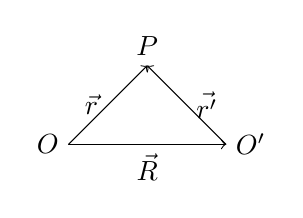
\begin{tikzpicture}[line cap=round,line join=round,scale=1]
        \coordinate (P) at (0, 1);
        \coordinate (O) at (-1, 0);
        \coordinate (Op) at (1, 0);

        \node[anchor=east] at (O) {\(O\)};
        \node[anchor=west] at (Op) {\(O'\)};
        \node[anchor=south] at (P) {\(P\)};

        \draw[->] (O) -- node[anchor=east] {\(\vec r\)} (P);
        \draw[->] (Op) -- node[anchor=west] {\(\vec {r'}\)} (P);
        \draw[->] (O) -- node[anchor=north] {\(\vec R\)} (Op);
    \end{tikzpicture}
\end{center}

Definiamo gli assi \(\hat{x}\), \(\hat{y}\) e \(\hat{z}\) per l'osservatore \(O\)
e \(\hat{u_1}\), \(\hat{u_2}\) e \(\hat{u_3}\) per \(O'\).
Chiaramente, questi versori sono dipendenti dal tempo per l'osservatore che non le usa (a meno
che i due osservatori non coincidano).
Dato questo sistema, abbiamo allora
\[
    \vec{r}'(t) = \sum_{i=1}^3 x_i'(t)\hat{u_i}(t)
\]
Abbiamo allora che
\begin{align*}
    \frac{d\vec{r}'(t)}{dt} &= \sum_{i=1}^3 \frac{dx_i'(t)}{dt} \hat{u_i}(t)
    + \frac{d\hat{u_i}(t)}{dt} x_i'(t) \\
    &= \sum_{i=1}^3 \frac{dx_i'(t)}{dt} \hat{u_i}(t)
    + \sum_{i=1}^3 \frac{d\hat{u_i}(t)}{dt} x_i'(t)
\end{align*}
The first term
\[
    \sum_{i=1}^3 \frac{dx_i'(t)}{dt} = \vec{r}'(t)
\]
is what \(O'\) perceives as the velocity, \(\vec{v}'(t)\).
Il termine dice di quanto cambiano le coordinate nel sistema di riferimento di \(O'\),
ossia la sua velocità.
Il secondo termine
\[
    \sum_{i=1}^3 \frac{d\hat{u_i}(t)}{dt} x_i'(t)
\]
compensa il primo.
Abbimo quindi che
\[
    \vec{v} = \vec{V} + \vec{v}'(t) + \sum_{i=1}^3 \frac{d\hat{u_i}(t)}{dt} x_i'(t)
\]

\stheorem{}{
    Esiste un vettore \(\vec{\omega}(t)\) tale che
    \[
        \frac{d\vec{u_i}}{dt} = \vec{w}(t) \wedge \vec{u_i}
    \]
}

Ciò vorrebbe dire che la terna di assi sta precedendo attorno alla direzione di \(\vec{\omega}\).
Tutte e 3 i versori stanno ruoando attorno allo stesso asse (infatti, non vi è l'indice \(i\) nel termine
\(\vec{\omega}\)). Tuttavia, il vettore \(\vec{\omega}\) stesso non è costante.
Per dimostrare ciò, dobbiamo dare la forma di \(\vec{\omega}\):
\[
    \vec{\omega}(t) = \frac{1}{2} \sum_{j=1}^3 \hat{u_j} \wedge \frac{d \hat{u_j}}{dt}
\]

Sostituendo otteniamo
\begin{align*}
    \vec{v} &= \vec{V} + \vec{v}'(t) + \sum_{i=1}^3 x_i'(\vec{\omega} \wedge \hat{u_i}) \\
    &= \vec{V} + \vec{v}'(t) + \vec{\omega} \wedge \sum_{i=1}^3 x_i'\hat{u_i} \\
    &= \vec{V} + \vec{v}'(t) + \vec{\omega} \wedge \vec{r}'(t)
\end{align*}

Verifichiamo che la forma di \(\vec{\omega}\) soddisfi la condizione data, quindi
\begin{align*}
    (\vec{\omega} \wedge \hat{u_i})_x &= \omega_y u_i^z - \omega_z u_i^y \\
    &= \frac{1}{2} \sum_{j=1}^3 \left\{ u_i^z \left[u_j^z \frac{du_j^x}{dt} - u_j^x \frac{du_j^z}{dt}\right]
     - u_i^y \left[u_j^x \frac{du_j^y}{dt} - u_j^y \frac{du_j^x}{dt}\right] \right\} \\
     &= \frac{1}{2} \sum_{j=1}^3 \left\{
        \frac{du_j^x}{dt} \left[
            u_i^z u_j^z + u_i^yu_j^y
        \right]
        - \frac{du_j^y}{dt} u_i^yu_j^x - \frac{du_j^z}{dt} u_i^zu_j^x
     \right\} \\
     &= \frac{1}{2} \sum_{j=1}^3 \left\{
        \frac{du_j^x}{dt} \left[
            \hat{u_i} \cdot \hat{u_j} - u_i^x u_j^x
        \right]
        - \frac{du_j^y}{dt} u_i^yu_j^x - \frac{du_j^z}{dt} u_i^zu_j^x
     \right\} \\
     &= \frac{1}{2} \sum_{j=1}^3 \left\{
        \frac{du_j^x}{dt} \left[
            \delta_{i,j} - u_i^x u_j^x
        \right]
        - \frac{du_j^y}{dt} u_i^yu_j^x - \frac{du_j^z}{dt} u_i^zu_j^x
     \right\} \\
     &= \frac{1}{2} \sum_{j=1}^3 \left\{
        \frac{du_j^x}{dt} \delta_{i,j} - u_j^x \left[
            u_i^x \frac{du_j^x}{dt} + \frac{du_j^y}{dt} u_i^y + \frac{du_j^z}{dt} u_i^z
        \right]
     \right\} \\
     &= \frac{1}{2} \frac{du_i^x}{dt} - \frac{1}{2} \sum_{j=1}^3
        u_j^x \left[
            u_i^x \frac{du_j^x}{dt} + \frac{du_j^y}{dt} u_i^y + \frac{du_j^z}{dt} u_i^z
        \right] \\
    &= \frac{1}{2} \frac{du_i^x}{dt} - \frac{1}{2} \sum_{j=1}^3
        u_j^x \left[
            \hat{u_i} \cdot \frac{d\hat{u_j}}{dt}
        \right]
\end{align*}

Siccome
\[
    0 = \frac{\hat{u_i}}{dt} \cdot \hat{u_j} + \hat{u_i} \frac{\hat{u_j}}{dt}
\]
Allora
\[
    \hat{u_i} \frac{\hat{u_j}}{dt} = - \frac{\hat{u_i}}{dt} \cdot \hat{u_j}
\]
e quindi
\begin{align*}
    (\vec{\omega} \wedge \hat{u_i})_x &= \omega_y u_i^z - \omega_z u_i^y \\
    &= \frac{1}{2} \frac{du_i^x}{dt} + \frac{1}{2} \sum_{j=1}^3
    u_j^x \left[
        \hat{u_j} \cdot \frac{d\hat{u_i}}{dt}
    \right] \\
    &= \frac{1}{2} \frac{du_i^x}{dt} + \frac{1}{2} \frac{du_i^x}{dt} \\
    &= \frac{du_i^x}{dt}
\end{align*}

Abbiamo quindi che
\[
    (\vec{\omega} \wedge \hat{u_i})_x = \frac{du_i^x}{dt}
    \qquad
    (\vec{\omega} \wedge \hat{u_i})_y = \frac{du_i^y}{dt}
    \qquad
    (\vec{\omega} \wedge \hat{u_i})_z = \frac{du_i^z}{dt}
\]

Tornando alla velocità,
\begin{align*}
    \vec{v} &= \vec{V} + \vec{v}' + \sum_{i=1}^3 x_i' (\vec{\omega} \wedge \hat{u_i}) \\
    &= \vec{V} + \vec{v}' + \vec{\omega} \wedge \sum_{i=1}^3 x_i' \hat{u_i} \\
    &= \vec{V} + \vec{v}' + \vec{\omega} \wedge \vec{r}'
\end{align*}

Troviamo ora la medesima relazione per l'accelerazione.
Siccome
\begin{align*}
    \frac{d\vec{v}'}{dt} &= \sum_{i=1}^3 \left[
        \frac{d^2 x_i'}{dt^2} \hat{u_i} + \frac{dx_i'}{dt} \frac{d\hat{u_i}}{dt}
    \right] \\
    &= \vec{a}' + \sum_{i=1}^3 \frac{dx_i'}{dt} \frac{d\hat{u_i}}{dt} \\
    &= \vec{a}' + \sum_{i=1}^3 \frac{dx_i'}{dt} (\vec{\omega} \wedge \hat{u_i}) \\
    &= \vec{a}' + \vec{\omega} \wedge \sum_{i=1}^3 \frac{dx_i'}{dt} \hat{u_i} \\
    &= \vec{a}' + \vec{\omega} \wedge \vec{v}'
\end{align*}
Possiamo trovare l'accelerazione
\begin{align*}
    \vec{a} &= \vec{A} + \frac{d\vec{v}'}{dt} + \frac{d\vec{\omega}}{dt} \wedge \vec{r}'
    + \vec{\omega} \wedge \frac{d\vec{r}'}{dt} \\
    &= \vec{A} + \vec{a}' + 2 \vec{\omega} \wedge \vec{v}' + \frac{d\vec{\omega}}{dt} \wedge \vec{r}'
    + \vec{\omega} \wedge (\vec{\omega} \wedge \vec{r}')
\end{align*}

L'ultimo termine \(\vec{\omega} \wedge (\vec{\omega} \wedge \vec{r}')\) è l'accelerazione centrifuga.
Il termine \(2 \vec{\omega} \wedge \vec{v}'\) è l'accelerazione di Coriolis.

\pagebreak

\section{Dinamica}

\textbf{Principio di relatività:}
Non esiste nessun esperimento in grado di decidere se noi siamo in quiete rispetto allo spazio assoluto
o ci stiamo muovendo in un moto rettilineo uniforme. Alternativamente, tutte le leggi della fisica sono equivalenti
indipendentemente dalla direzione dell'esperimento e dal sistema di riferimento (inerziali).

Il principio della relavitià risale a Galileo nel dialogo, 1632.

\textbf{Leggi di Newton:}
\begin{enumerate}
    \item un corpo mantiene il prorpio stato di quiete
    o di moto rettilineo uniforme
    se non agiscono forze esterne;
    \item \(\vec{F} = m\vec{a}\);
    \item se un corpo \(1\) esercita una forza \(\vec{F_{1,2}}\) su un corpo \(2\),
    allora il corpo \(2\) esercita una forza \(\vec{F_{2,1}} = -\vec{F_{1,2}}\)
    sul corpo \(1\).
\end{enumerate}

La prima è in realtà un caso particolare della seconda.

L'espressione \(\vec{F} = m\vec{a}\) è una relazione fra causa ed effetto. La forza è la causa,
che determina direttamente le accelerazioni.

Tuttavia, è necessario prima definire il concetto di massa.
Ciò può essere fatto con una serie di esperimenti e osservazioni.
Consideriamo due palline attaccate ai capi di una molla:
\begin{enumerate}
    \item \(\vec{a_1} \neq 0 \implies \vec{a_2} \neq 0\);
    \item \(\vec{a_1}\) e \(\vec{a_2}\) hanno verso opposto;
    \item il rapporto \[
        \frac{|\vec{a_1}|}{|\vec{a_2}|}
    \]
    è indipendente dalla interazione, bensì solamente dalle caratteristiche
    delle particelle;
    \item se i due corpi sono dello stesso materiale, ma di volumi diversi,
    allora
    \[
        \frac{|\vec{a_1}|}{|\vec{a_2}|} = \frac{V_2}{V_1}
    \]
\end{enumerate}
Allora, per ogni coppia di corpi, definiamo
\[
    \frac{m_2}{m_1} = \frac{|\vec{a_1}|}{|\vec{a_2}|}
\]
Dobbiamo quindi scegliere una massa di base sulla quale basare le altre misure.
Sperimentalmente, troviamo anche che \(\vec{F_1} + \vec{F_2} = m(\vec{a_1} + \vec{a_2})\).

Conservazione della quantità di moto
\[
    \vec{Q} = m\vec{v}
\]
e
\[
    \vec{Q} = \vec{Q_1} + \vec{Q_2} = m_1\vec{v_1} +  m_2\vec{v_2}
\]
La derivata della quantità di moto è data da
\[
    \frac{d\vec{Q}}{dt} = m_1 \frac{d\vec{v_1}}{dt} + m_2 \frac{d\vec{v_2}}{dt}
    = m_1 \vec{Q_1} + m_2 \vec{Q_2}
\]
Il vettore della quantità di moto nel tempo, di due moti che interagiscono fra di loro,
è sempre il medesimo, e quindi si conserva.

\pagebreak

\section{Forze elastiche (Legge di Hooke)}

\stheorem{Legge di Hooke}{
    La forza elastica è data da
    \[
        \vec{F_e} = -k \vec{x}
    \]
    dove \(\vec{x}\) è il vettore di elongazione e
    \(k\) è la costante elastica.
    Il segno negativo indica che la forza è una forza di richiamo.
}

In realtà questa è un'approssimazione lineare,
e presume quindi che lo spostamento sia piccolo.

Spesso viene indicata la quantità di pulsazione
\[
    \omega^2 = \frac{k}{m}
\]
Il significato deriva dalla soluzione dell'equazione differenziale \(ma_x = F_x\),
\[
    \frac{d^2 x}{dt^2} = -\omega^2 x % TODO
\]
da cui deriva
\[
    x(t) = A \cos(\omega t + \varphi)
\]

%\section{Pendolo}
%
%% TODO disegno pendolo l, m
%
%\begin{center}
%    \begin{tikzpicture}[line cap=round,line join=round,scale=2.5]
%        \node[left] at (0,1) {\(C\)}; 
%        \fill (0,1) circle (0.75pt);
%
%        \draw[-, thick] (0,1) -- (0.25,0.5);
%        \fill (0.25,0.5) circle (1pt);
%        \node[below right] at (0.25,0.5) {\(m\)}; 
%        \node[above right] at (0.125,0.75) {\(l\)}; 
%
%        \draw[->, thin, dashed] (0.25,0.5) -- (0.25,0.25);
%
%        \draw[->] (0,0) -- (0,1.1);
%        \draw[dashed] (-0.4,0.54) arc (-120:-60:0.75 and 0.75);
%    \end{tikzpicture}
%\end{center}
%
%Chiaramente, \(\vec{F} = -mg \hat{z}\).
%Il corpo è vincolato ad un percorso sul cerchio con centro il perno.
%La posizione del punto è univocamente determinata dal raggio e dal suo angolo \(\theta\)
%rispetto al perno.
%Dal disegno notiamo che
%\[
%    F_N = T - mg \cos\theta
%\]
%mentre
%\[
%    F_T = -mg\sin\theta
%\]
%in quanto la tensione del filo non ha componenti tangenziali.
%Sappiamo che per un moto arbitrario, la sua accelerazione può sempre essere
%scritta in termini dell'accelerazione tangenziale e quella normale \(\vec{a} = \vec{a_T} + \vec{a_N}\).
%Allora,
%\[
%    \begin{cases}
%        m\frac{v^2}{R} = T - mg\cos\theta \\
%        \frac{dv}{dt} = -g\sin\theta
%    \end{cases}
%\]
%in questo caso il raggio di curvatura \(R\) è precisamente il raggio della circonferenza.
%La distanza percorsa dal punto è \(s=l\Delta \theta\) e quindi
%\[
%    v = l \frac{d\theta}{dt}
%\]
%Sostituendo, troviamo la tensione del filo in funzione di \(\theta\),
%dove \(\theta\) viene data dalla seconda equazione
%\[
%    \begin{cases}
%        \frac{d\theta^2}{dt^2} = -\frac{g}{L}\sin\theta
%    \end{cases}
%\]
%
%Possiamo notare che il primo termine della tensione
%si annulla ai due estremi. Il secondo termine
%diventa negativo quando la pallina si trova sopra la semicirconferenza.
%Infatti, in tale caso la tensione è negativa, e il cavo esercita tensione opposta
%rispetto all'altro caso, in quanto deve contrastare il tentativo della pallina di accorciarlo.
%Se la velocità iniziale è sufficientemente alta, la tensione è comunque positiva
%se la pallina si trova nella parte superiore della circonferenza (come quando esegue un giro completo),
%in tal caso la pallina sta comunque cercando di allungare il cavo.
%
%Troviamo quindi la funzione \(\theta\). Per farlo, notiamo che
%per piccoli angoli l'equazione è approssimativamente una funzione lineare.
%Quindi,
%\begin{align*}
%    \theta = \theta_0 \cos(\omega t + \varphi), \quad \omega = \sqrt{\frac{g}{l}}
%\end{align*}
%con \(\varphi = 0\) (siccome la velocità iniziale è zero, il vincolo annulla la costante).
%L'equazione senza l'approssimazione lineare non ha forma chiusa.
%
%L'equazione del pendolo
%\[
%    \frac{d^2\theta}{dt} = -\sin\theta
%\]
%può essere scomposta in due equazioni differenziali del primo ordine
%importando \(x = y\) e \(y = \frac{d\theta}{dt}\)
%e quindi
%\[
%    \begin{cases}
%        \frac{dx}{dt} = y \\
%        \frac{dy}{dt} = -\sin x
%    \end{cases}
%\]

\section{Carrucola con due masse}

\begin{center}
    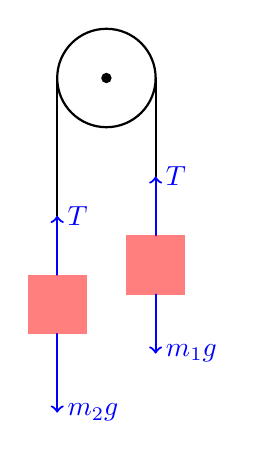
\begin{tikzpicture}[line cap=round,line join=round,scale=2.5]
        \fill (0,0) circle (0.75pt);

        \draw[thick] (0.25,0) arc (0:360:0.25);
        \draw[-, thick] (0.25,0) -- (0.25,-0.5);
        \draw[-, thick] (-0.25,0) -- (-0.25,-0.7);

        \draw[->, thick, blue] (0.25,-0.8) -- (0.25,-0.5) node[right] {\(T\)};
        \draw[->, thick, blue] (-0.25,-1.0) -- (-0.25,-0.7) node[right] {\(T\)};

        \fill [red, opacity=0.5] (0.1,-0.8) rectangle ++(0.3,-0.3);
        \fill [red, opacity=0.5] (-0.4,-1) rectangle ++(0.3,-0.3);

        \draw[->, thick, blue] (0.25,-1.1) -- (0.25,-1.4) node[right] {\(m_1g\)};
        \draw[->, thick, blue] (-0.25,-1.3) -- (-0.25,-1.7) node[right] {\(m_2g\)};
    \end{tikzpicture}
\end{center}

Abbiamo \(a_2 = -a_1\)
\[
    \begin{cases}
        m_1a_1 = T-m_1g \\
        -m_2a_1 = T-m_2g
    \end{cases}
\]

\pagebreak

\section{Attriti}

Se la velocità di un oggetto è nulla, la forza di attrito esercitata su di esso è
anch'essa nulla.
In caso contrario, per velocità relativamente basse, 
la forza è data da \(\vec{F_a} = -\gamma\vec{v}\).

In un liquido con viscosità \(\eta\), dalla legge di Stokes,
una sfera di raggio \(a\) (con superficie perfettamente rigida che non ha
interazioni con il fluido) ha coefficiente di attrito
\[
    \gamma = 6\pi\eta a
\]

Consideriamo il moto di un oggetto affetto solamente dalla forza di attrito.
Allora \(-\gamma v = ma\). L'equazione differenziale che governe il moto è quindi
\[
    \frac{dv}{dt} = -\frac{\gamma}{m}v
\]
e quindi
\[
    v(t) = v_0e^{\lambda t}, \quad \lambda = -\frac{\gamma}{m}
\]
e il moto
\[
    x(t) = \frac{v_0}{\lambda} e^{\lambda t} + x_0, \quad \lambda = -\frac{\gamma}{m}
\]
Ma siccome \(x(0) = 0\), allora \(x_0 = - \frac{v_0}{\gamma}\)
e quindi
\[ x(t) = v_0 \frac{m}{\gamma} \left[1 - e^{-\frac{\gamma}{m}t}\right] \]
La velocità tende a zero senza toccarlo, ma la posizione è finita.

Un oggetto che cade ha forza \(F_z = -mg - \gamma v_z = ma_z = m\frac{dv_z}{dt}\)
E quindi l'equazione differenziale è
\[
    \frac{dv_z}{dt} = -g - \frac{\gamma}{m} v_z
\]
e quindi
\[
    v_z(t) = g\frac{m}{\gamma} \left[e^{-\frac{\gamma}{m}t} - 1\right]
\]

Un oggetto su un piano al quale viene applicata una forza, subirà la forza inversa
dell'attrito dove \(|\vec{F_A}| = \mu R\)
dove \(\mu\) è un coefficiente adimensionale che dipende dalla natura delle due superfici
e \(R\) è la reazioe vincolare. \textbf{NON} è proporzionale alla massa, ma la reazione vincolare
è certamente legata alla massa. La reazione vincolare deve essere tale da compensare esattamente
la forza peso. Quindi, la reazione vincolare è \(mg\). È importante notare che potrebbe
esserci il caso \(g=0\), dove non vi è attrito, e quindi non è proporzionale alla massa.
i coefficienti di attrito di distinguono in quello statico e quello dinamico.
Quello statico è legato alla minima forza che bisogna applicare per mettere in moto un oggetto,
mentre quello dinamico è legato al movimento dell'oggetto stesso.
In generale \(\mu_S > \mu_D\).

Il coefficiente di attrito deriva dal fatto che le superfici di contatto siano
ruvide; solamente una piccola porzione delle due superfici macroscopiche sono effettivamente a contatto.
Questo è anche il motivo per il quale il coefficiente di attrito statico è generalmente maggiore
di quello dinamico, ossia il fatto che bisogna applicare sufficiente energia per rompere
i punti di blocco fra le due superfici. I coefficienti di attrito
non dipendono dall'area di appoggio (infatti, a parità di massa ma differenza di area
superficiale i coefficienti di attrito sono equivalenti).


Nel piano inclinato il corpo si muove solamente se \(mg\sin\alpha > \mu_S mg\cos\alpha\)
ossia \(\tan \alpha > \mu_S\).
Una volta in movimento l'accelerazione è data da \(g\cos\alpha\left[\tan\alpha-\mu_D\right]>0\).
Questo tipo di attrito non dipende dalla velocità.

\pagebreak

\section{Forze apparenti}

Consideriamo osservatori \(O\) e \(O'\) dove \(O\)
possiede un sistema di riferimento inerziale, e quindi può necessariamente
usare le leggi della dinamica. Abbiamo quindi la relazione
\begin{align*}
    \vec{F} = m\vec{a} = m \left[\vec{A} + \vec{a}' + 2 \vec{\omega} \wedge \vec{v}' + \frac{d\vec{\omega}}{dt} \wedge \vec{r}'
    + \vec{\omega} \wedge (\vec{\omega} \wedge \vec{r}') \right]
\end{align*}

\sdefinition{Forza apparente}{
    La \emph{forza apparente} è data da
    \[
        \vec{F}_\text{app} = -m\vec{a} = m \left[\vec{A} + \vec{a}' + 2 \vec{\omega} \wedge \vec{v}' + \frac{d\vec{\omega}}{dt} \wedge \vec{r}'
        + \vec{\omega} \wedge (\vec{\omega} \wedge \vec{r}') \right]
    \]
    e quindi
    \[
        \vec{F} + \vec{F}_\text{app} = m \vec{a'}
    \]
}

In tal maniera, l'osservatore del sistema non inerziale può usare le leggi di Newton,
purché oltre alle forze vere vengano aggiunge le forze apparenti.
In questo caso, le forze non hanno responsabile, ma solamente perché il sistema di riferimento
non è inerziale.
Le forze di Coriolis e quella centrifuga mantengono lo stesso nome.
Quando una macchina frena e io vengono spinto in avanti, la forza è apparente
se descrivo il sistema di riferimento come non-inerziale.

Nel caso della terra, la forza di Coriolis è data da
\[
    \vec{F}_c = -m\vec{\omega} \wedge (\vec{\omega} \wedge \vec{r})
\]
È sempre ortogonale all'asse di rotazione (l'equatore).
Il suo modulo è dato da
\[
    F_c = m\omega^2 R \sin\alpha
\]
dove \(\alpha\) è l'angolo compreso e \(R\) il raggio della terra.
La componente verticale è \(m \omega^2 R \sin^2\alpha\).

\sexample{Esempio}{
    Montiamo una carrucola con un peso al soffitto di un ascensore che sta salendo con accelerazione \(A\).
    Tiriamo la corda verso il basso per far salire il peso con una velocità costante
    (rispetto a noi).
    Sul peso agisce la forza peso \(-mg\) e la tensione del filo \(T\).
    Siccome sto descrivendo il peso in un sistema di riferimento non inerziale, avrò
    una forza apparente che agisce su di lei, ossia \(-mA\).
    Quindi
    \[
        F = -mg + T - mA = 0
    \]
    in quanto il moto si muove di moto rettilineo uniforme nel mio sistema.
    Quindi la tensione del filo
    \[
        T = m(g+A)
    \]
    (viene sottoposto ad una tensione maggiore per via del moto accelerato dell'ascensore).
    Quindi, a causa dell'accelerazione verso l'alto devi esercitare più forza per far salire il peso.
}

\sexample{Esempio}{
    Consideriamo un osservatore \(O'\) solidale ad un asta che ruota con una certa velocità
    angolare \(\omega\). Sull'asta, inseriamo un anello scorrevole inizialmente ad una certa distanza
    \(l_0\) dall'origine.
    Perché l'anello si allontana dall'origine?
    A parte le forze che vincola l'anello a stare sull'asta, l'osservatore non inerziale,
    solidale con l'asta, vede che sul corpo agisce una forza apparente (centrifuga).
    Questa forza apparente centrifuga è diretta nella direzione che si allontana dall'origine
    stando sull'asta. Il suo modulo è dato da
    \[
        m\omega^2 x
    \]
    dove \(c\) è la distanza.
    Per l'osservatore
    \[
        m \frac{d^2x}{dt^2} = m\omega^2 x
    \]
    che ricorda l'equazione dell'oscilaltore armonico. La soluzione è
    \[
        x(t) = C_1e^{\omega t} + C_2e^{-\omega t}
    \]
    Le condizioni iniziali dell'anello sono \(x(0)=l_0\)
    e \(v(0) = 0\).
    Quindi,
    \[
        \begin{cases}
            C_1 + C_2 = l_0 \\
            0 = \omega(C_1 - C_2)
        \end{cases}
        \implies a = b = \frac{l_0}{2}
    \]
    e allora
    \[
        x(t) = l_0 \cosh(\omega t)
    \]
}

\stheorem{}{
    Il \textit{teorema dell'impulso}
    dice che il cambiamento della quantità di modo in un impulso
    è pari alla forza applicata per il tempo passato
    \[
        \vec{I} \triangleq \int_{t_0}^{t_1} \vec{F}\,dt
        = m\left[\vec{v}(t_2) - \vec{v}(t_1)\right]    
    \]
}

Quindi, l'impulso di una forza è la differenza di quantità di moto \(\Delta \vec{Q}(t)\).

\subsection{Sistemi a massa variabile}

Se la massa di un oggetto è esplicitamente dipendente dal tempo \(M(t)\),
l'equazione di Newton non è \(\vec{F} = M(t) \vec{a}\).

Immaginiamo di porre delle palline per terra e coprirle con una scatola.
Trasciniamo la scatola con velocità \(v\). Ad un certo punto, la scatola comincierà a trascinare
anche le palline al suo interno.
Usiamo il teorema dell'impulso per dire che la differenza di quantità di moto è l'integrale
della forza.
In questo caso la forza è quindi data da \(F = \frac{dM}{dt} v\). Anche se la velocità è costante,
la forza deve aumentare per mantenere il medesimo moto.
L'accelerazione è nulla ma la forza non è nulla.

Una generalizzazione per descrivere sia i casi a massa costante che a massa variabile
è quella di scrivere
\[
    \vec{F} = \frac{d\vec{Q}}{dt}, \quad \vec{Q} = M(t)\vec{v}(t)
\]
Quindi,
\[
    \vec{F} = \begin{cases}
        M \vec{a} & M \text{ costante}\\
        \frac{dM}{dt}\vec{v} + M\vec{a} & M \text{ non costante}
    \end{cases}
\]

% massa gravitazionale =? massa inerziale

\pagebreak

\section{Energia}

%\sdefinition{Lavoro}{
%    Se la forza \(\vec{F}\) è costante,
%    il \emph{lavoro} è definito come
%    \[
%        L = \vec{F} \cdot \vec{s}
%    \]
%    dove \(\vec{s}\) è lo spostamento,
%    con unità di misura in Joule. % = newton * metro
%}
%
%Notiamo che la traiettoria è indipendente.
%
%Se la forza non è costante, dividiamo la traiettoria in tanti intervalli
%di lunghezza \(\Delta s\). La forza è essenzialmente costante per ogni intervallo di lunghezza
%sufficientemente piccola.
%Allora definiamo il lavoro come
%\[
%    \sum_{i=1}^N L_i = \sum_{i=1}^N \vec{F_i} \cdot \Delta s_i
%\]
%e quindi
%\[
%    L = \lim_{N\to\infty} \sum_{i=1}^N \vec{F_i} \cdot \Delta s_i = \int_C \vec{F} \,d\vec{s}
%\]
%dove \(C\) è il percorso.

%\sdefinition{Potenza}{
%    La \emph{potenza} è definita dalla quantità
%    \[
%        \frac{dL}{dt} = \vec{F}(t) \cdot \vec{v}(t)
%    \]
%    con unità di misura in Watt.
%}
%
%La forma è ottenuta facendo
%\[
%    \lim_{h\to0} \frac{L(t+h)-L(t)}{h}
%    \lim_{h\to0} = \frac{\vec{F} \cdot \vec{s}}{h} = \vec{F} \cdot \vec{v}
%\]

%\stheorem{Teorema delle forze vive / dell'energia cinetica}{
%    \[
%        L = E_C(t_2) - E_C(t_1)
%    \]
%}
%
%\sproof{}{
%    Accoppiamo la definizione di potenza con con \(\vec{F}=m\vec{a}\) e troviamo
%    \begin{align*}
%        \frac{dL}{dt} &= m\vec{a}\vec{v} = m\vec{v}\frac{d\vec{v}}{dt}
%    \end{align*}
%    Siccome
%    \[
%        \frac{d}{dt}\left(\vec{v}\cdot \vec{v}\right) = 2\vec{v}\frac{d\vec{v}}{dt}
%    \]
%    troviamo allora
%    \begin{align*}
%        \frac{dL}{dt} &= m \frac{1}{2} \frac{d(\vec{v} \cdot \vec{v})}{dt}
%        = \frac{d}{dt} \left(\frac{1}{2} m v^2(t)\right)
%    \end{align*}
%    Dal teorema fondamentale del calcolo
%    \[
%        L = \integral[t_1][t_2][\frac{dL}{dt}][t]
%        = \integral[t_1][t_2][\frac{d}{dt}E_c][t]
%        = E_C(t_2) - E_C(t_1)
%    \]
%}

Le forze vincolari sono sempre ortogonali al vincolo, e quindi non compiono mai lavoro.

Nel caso speciale in cui la forza è costante, abbiamo
\[
    L = \int_C \vec{F}\,d\vec{s} = \vec{F} \int_C d\vec{s}
\]
In questo caso bisogna solamente sommare tutti i vettori
della divisione infinitesimale. La somma di tali vettori che il vettore dal
primo punto \(A\) all'ultimo punto \(B\).
\[
    L = \vec{F} \cdot \vec{AB}
\]

Nel caso in cui la traiettoria sia lineare abbiamo
\[
    L = \int_C \vec{F}\,d\vec{s} = \integral[x_A][x_B][F(x)][x]
\]

Le forze vincolare sono sempre ortogonali allo spostamento e non rientrano nel lavoro.

Viene spesso definitva la funzione \(U(x)\)
tale che
\[
    F_x = -\frac{dU}{dx}
\]
In tal caso
\[
    L_{AB} = \integral[x_A][x_B][F_x][x] = U(x_A) - U(x_B)
\]
Siccome \(L_{AB} = E_C(B) - E_C(A)\), otteniamo che
\[
    E_C(A) + U_A = E_C(B) + U_B
\]
La funzione \(U\) è detta l'energia potenziale.

\sdefinition{Energia meccanica}{
    L'\textit{energia meccanica} è data da
    \[
        E_C + U
    \]
}

L'energia meccanica viene conservata (per tutte le forze conservative, cioè dove è possibile
definire una tale funzione \(U\)).

Le forze vincolari non sono conservative, ma non compiono lavoro quindi possiamo ignorarle.
Le forze posizionali sono conservatrici (deve dipendere solamente dalla posizione istantanea).
La forza di attrito viscoso, per esempio, non dipende solo dalla posizione e quindi non potrà mai esistere
una funzione \(U\).

\pagebreak

\subsection{Sistemi tridimensionali}

Supponiamo che le forze siano posizionarie.

Dobbiamo definire le derivate per funzioni tridimensionali, dove chiaramente
ogni direzione ha una derivata propria.
\[
    \lim_{h \to 0} \frac{f(\vec{r} + h\vec{d}) - f(\vec{r})}{h}
\]
Notiamo che
questa si può esprimere in termini come combinazione lineare delle derivate parziali
\[
    \vec{d} \begin{pmatrix}
        \frac{\partial f}{\partial x} \\
        \frac{\partial f}{\partial y} \\
        \frac{\partial f}{\partial z}
    \end{pmatrix}
    = \vec{d} \nabla f
\]
%\begin{align*}
%    \phantom{ } &= \lim_{h \to 0} \hat{x}\frac{f_x(x + h\vec{d}) - f_x(\vec{x})}{h} \\
%    &=
%    \lim_{h \to 0} {f(x + h\vec{d}, y + h\vec{d}, z + h\vec{d}) - f(x,y,z)}{h} \\
%    &= 
%    \lim_{h \to 0} {f(x + h\vec{d}, y + h\vec{d}, z + h\vec{d}) - f(x,y,z) + f(x,y+ h\vec{d},z+ h\vec{d}) - f(x,y+ h\vec{d},z+ h\vec{d})}{h} \\
%    &= 
%    \lim_{h \to 0}
%    {f(x + h\vec{d}, y + h\vec{d}, z + h\vec{d}) - f(x,y,z)}{h}
%    +
%    {f(x + h\vec{d}, y + h\vec{d}, z + h\vec{d}) - f(x,y,z)}{h}
%\end{align*}

%\subsection{Forze conservatrici}

%\sdefinition{Forza conservativa}{
%    Si definisce la \emph{forza conservative} come una forza posizionale e tale
%    che
%    \[
%        \vec{F}(\vec{r}) = -\nabla U(\vec{r})
%    \]
%}
%
%Non tutte le forze posizionali sono conservative; la condizione del gradiente
%deve venire rispettata.
%
%\stheorem{Lavoro di una forza conservativa}{
%    Consideriamo un corpo soggetto a solamente forze conservative \(\vec{F}(\vec{r})\).
%    Allora, \(L = U(A) - U(B)\).
%}
%
%\sproof{Lavoro di una forza conservativa}{
%    Considera il lavoro
%    \begin{align*}
%        L &= \sum_{i=1}^N \vec{F_i} \cdot \Delta \vec{s_i} \\
%        &= \sum_{i=1}^N \vec{F_i} \cdot |\Delta \vec{s_i}| \frac{\Delta \vec{s_i}}{|\Delta \vec{s_i}|}
%    \end{align*}
%    L'ultimo termine è un versore, e quindi abbiamo la derivata direzionale
%    \begin{align*}
%        L &= \int_C \vec{F} \,d\vec{s} \\
%        &= - \sum_{i=1}^N \left(
%            \nabla U_i \cdot \vec{m_i}
%        \right) |\Delta \vec{s_i}| \\
%        &= - \sum_{i=1}^N \frac{
%            U(\vec{r_{i-1}} + \Delta \vec{s_i}) - (\vec{r_{i-1}})
%        }{
%            |\Delta \vec{s_i}|
%        } |\Delta \vec{s_i}| \\
%        &= - \left[
%            U(\vec{r_1}) - U(\vec{r_0}) + U(\vec{r_2}) - U(\vec{r_1})
%            + \cdots + U(\vec{r_N}) - U(\vec{r_{N-1}})
%        \right] \\
%        &= U(\vec{r_0}) - U(\vec{r_N}) \\
%        &= U(A) - U(B)
%    \end{align*}
%}

%Mettendo il teorema assieme a quello delle forze vive, otteniamo la conservazione dell'energia meccanica.
%
%\stheorem{Conservazione dell'energia meccanica}{
%    Per le forze conservative
%    \[
%        E_C(A) + U(A) = E_C(B) + U(B)
%    \]
%}
%
%Per la forza peso \(F_z = -mg = -\nabla U\) abbiamo \[U(z) = mgz\]
%
%Per la forza elastica \(F_x = -kx = -\nabla U\) abbiamo \[U(x) = \frac{1}{2}kx^2\]

%\subsection{Forze centrali}

%\sdefinition{Forza centrale}{
%    Le forze centrali sono delle forze posizionali il cui modulo
%    \(\vec{F}(\vec{r}) = f(r)\) dipende esclusivamente dalla distanza,
%    e sono dirette come \(\vec{r}\) (versore radiale).
%}
%
%\stheorem{}{
%    Ogni forza centrale è conservativa.
%}
%
%\sproof{}{
%    Consideriamo \(\vec{F}(\vec{r}) = -\nabla U\).
%    Vogliamo trovare
%    \[
%        \frac{\partial U}{\partial x}
%    \]
%    la componente \(x\) è presente in \(\vec{r}\).
%    Allora \(r=\sqrt{x^2 + y^2 + z^2}\). Quindi,
%    \begin{align*}
%        \frac{\partial U}{\partial x} &= \frac{dU}{dr} \frac{\partial r}{\partial x} \\
%        &= \frac{dU}{dr} \frac{x}{r}
%    \end{align*}
%    Le altre variabili sono analoghe.
%    Allora il gradiente di \(U\) è dato da
%    \begin{align*}
%        \nabla U(r) &=
%        \frac{dU}{dr} \frac{x}{r} \hat{x} +
%        \frac{dU}{dr} \frac{y}{r} \hat{y} +
%        \frac{dU}{dr} \frac{z}{r} \hat{z} \\
%        &= \frac{dU}{dt} \hat{r}
%    \end{align*}
%    La forza centrale è quindi proprio una funzione
%    \[
%        f(r) = - \frac{dU}{dr}
%    \]
%    e quindi
%    \[
%        \vec{F} = f(r) \hat{r} = -\nabla U
%    \]
%}

\pagebreak

\section{Esercizi}

\subsection{17 ottobre}

\sexercise{Un corpo viene lasciato cadere da una certa altezza
con velocità iniziale nulla: quanto tempo \(t\) si deve attendere perché
a parte da quell'istante il corpo percorra uno spazio di \(s= 20m\)
nel tempo \(\tau = 1s\)}{
    La funzione di caduta è data da \(s = \frac{1}{2}at^2 + v_0t + s_0\).
    Abbiamo allora 
    \begin{align*}
        20 &= \integral[t][t+1][v_0 + ax][x] \\
        20 &= \frac{1}{2}a{(t+1)}^2 - \frac{1}{2}at^2 \\
        40 &= a{(t+1)}^2 - at^2 \\
        40 &= a(t^2 + 2t + 1) - at^2 \\
        40 &= at^2 + 2at + a - at^2 \\
        40 &= 2at + a \\
        40 - a &= 2at \\
        t &= \frac{40 - a}{2a}
    \end{align*}
}

\sexercise{Il moto nel piano \(x\), \(y\) di una particella è definito da
\[
    \begin{cases}
        x = \alpha t^2  + \beta t \\
        y = \alpha t^2  - \beta t
    \end{cases}
\]
Con \(\alpha = 0.1 m/s^2\) e \(\beta = 1 m/s\).
Si calcolino i moduli della velocità e dell'accelerazione
all'istante \(\tau = 10s\)}{
    Calcoliamo le velocità
    \[
        \begin{cases}
            v_x = \frac{dx}{dt} = 2\alpha t + \beta \\
            v_y = \frac{dy}{dt} = 2\alpha t - \beta
        \end{cases}
    \]
    e le accelerazioni
    \[
        \begin{cases}
            a_x = \frac{dv_x}{dt} = 2\alpha \\
            a_y = \frac{dv_y}{dt} = 2\alpha
        \end{cases}
    \]
    Il modulo della velocità è pari a
    \begin{align*}
        |v| = \sqrt{v_x^2 + v_y^2}
        &= \sqrt{4\alpha^2 t^2 + 4\alpha\beta t + \beta^2 + 4\alpha^2 t^2 - 4\alpha\beta t + \beta^2} \\
        &= \sqrt{8\alpha^2 t^2 + 2\beta^2}
    \end{align*}
    Il modulo della accelerazione è pari a
    \begin{align*}
        |a| = \sqrt{8}\alpha
    \end{align*}
}

\sexercise{Un'automobile in moto con velocità di modulo \(v_0\)
comincia a frenare e, muovendosi di moto rettilineo, si arresta
in uno spazio \(l\).
Si determini l'accelerazione scalare media di frenamento nei tre casi seguenti:
}{
    \begin{enumerate}
        \item l'accelerazione scalare ha valore \(A\) costante nel tempo:
            Abbiamo che \(v = v_0 + At\) e \(s = v_0t + \frac{1}{2} A t^2\).
            Chiamiamo allora \(t^*\) il tempo per cui \(v=0\).
            Allora \(v_0 + At^* = 0 \implies t^* = - \frac{v_0}{A}\).
            %Allora \(l= v_0t^* + \frac{1}{2}At^*^2\)
            Sostituiamo \(t^*\) nell'accelerazione media
            \[
                a_m = \frac{v - v_0}{-t^*} = \frac{v_0}{-t^*} = A
            \]
        \item l'accelerazione dipende dalla velocità scalare con la legge:
        \(a = b(v + v_0)\). Dobbiamo trovare
        \begin{align*}
            \frac{dv}{dt} &= b(v + v_0)
        \end{align*} 
        quindi
        \begin{align*}
            v = ce^{\xi t} + V \qquad \frac{dv}{dt} = c\xi e^{\xi t} + V
        \end{align*}
        con \(V = -v_0\), \(\xi = b\) e \(c\) libera.
        Siccome \(v(0) = v_0\) allora \(c = 2v_0\) e quindi \(v(t) = v_0(2e^{b t} - 1)\).
        Per calcolare la posizione integriamo nuovamente
        \[
            \frac{ds}{dt} = v_0(2e^{bt} - 1)
        \]
        e allora
        \[
            s(t) = \frac{2v_0}{b}e^{bt} -v_0 t + s_0
        \]
        Siccome \(s(0) = 0 = -\frac{2v_0}{b}\), troviamo
        \[
            s(t) = \frac{2v_0}{b}(e^{bt} - 1) - v_0t
        \]
        Per il tempo di arresto abbiamo che \(v_0(2e^{bt} - 1) = 0\)
        e quindi \(t^* = - \frac{\ln 2}{b}\).
        Quindi \begin{align*}
            l &= s(t^*) = \frac{v_0}{b}\left(\ln 2 - 1\right) \\
            b &= \frac{v_0}{l} \left(\ln 2 - 1\right)
        \end{align*}
        Quindi l'accelerazione media è data da
        \[
            a_m = \frac{-v_0}{t^*} = \frac{v_0^2}{t} \frac{\ln 2 - 1}{\ln 2}
        \]
        \item l'accelerazione varia linearmente nel tempo \(a = \gamma t\):
            Integrando dobbiamo troviamo
            \begin{align*}
                v(t) &= v_0 + \frac{1}{2}\gamma t^2 \\
                s(t) &= v_0 t + \frac{1}{6}\gamma t^3
            \end{align*}
            siccome \(s_0 = 0\).
            \(\cdots\)
            Infine,
            \[
                a_m = \frac{2v_0^2}{3l}
            \]
    \end{enumerate}
}

\sexercise{Un corpo di piccole dimensioni
    viene lanciato verticalmente verso l'alto all'istante \(t=0\).
    Nella fase di salita e in quella successiva di discesa, l'oggetto passa dalla quota
    \(h\), rispetto alla posizione di lancio, agli istanti \(t_1\) e \(t_2\), rispettivamente:
    si dimostri che vale la relazione \(t_1t_2 = 2h/g\). Si trascuri l'effetto della
    resistanza dell'aria sul moto del corpo.}{
    La legge oraria è data da \(s(t) = v_0t + \frac{1}{2}at^2\).
    Dal testo abbiamo \(s(t_1) = s(t_2) = h\)
    e \(at^2 - 2v_0t + 2h = 0\).
    Le soluzioni sono
    \[
        t_1t_2 = \frac{v_0}{a} \pm \sqrt{\frac{v_0^2}{a^2} - \frac{2h}{g}}
    \]
    e quindi
    \[
        t_1t_2 = \frac{2h}{g}
    \]
}

\sexercise{Un corpo viene lanciato orizzontalmente
da altezza \(h_0\) rispetto al suolo, con velocità \(v_0\).
Trascurando la resistenza dell'aria, si calcoli:}{
    \begin{enumerate}
        \item la componente tangenziale \(a_T\) e quella normale \(a_N\)
        dell'accelerazione del corpo rispetto alla traiettoria, in un generico
        punto di altezza \(h\):
        abbiamo che \(P_0 = (0, h_0)\) e \(\vec{v_0} = (v_0, 0)\).
        Allora
        \[
            \begin{cases}
                a_x = 0 \\
                a_z = -g
            \end{cases}
        \]
        e
        \[
            \begin{cases}
                v_x = v_0 \\
                v_y = -gt
            \end{cases}
        \]
        e infine
        \[
            \begin{cases}
                x = v_0t \\
                z = h_0 - \frac{1}{2}gt^2
            \end{cases}
        \]
        Il vettore tangente è il vettore della velocità.
        Vogliamo trovare la legge che lega il tempo all'asse \(z\).
        Quindi \(\vec{v} = v_0\hat{x} - \sqrt{2g(h_0-z)}\hat{z}\)
        e \(|v| = \sqrt{v_0^2 + 2g(h_0 - z)}\).
        Se considiamo \(\alpha\) come l'angolo fra il vettore di gravitazione
        (asse x) e il vettore normale,
        \[
            \cos\alpha = \frac{\vec{v}\cdot\hat{x}}{|v|}
            = \frac{v_0}{\sqrt{v_0^2 + 2g(h_0 - z)}}
        \]
        che dipende da \(z\).
        Proiettiamo la gravità sulle sulle componenti, quindi
        \(a_T = g\sin\alpha\) e \(a_N = g\cos\alpha\), che si calcola facilmente
        con la relazione pitagorica del seno e coseno.
        \item lo spazio \(s\) percorso dal corpo dall'istante
        di lancio \(t=0\) a quello in cui tocca il suolo:
        \[
            \integral[0][\text{gittata}][\sqrt{1 + {\left(\frac{dz}{dx}\right)}^2}][x]
        \]
    \end{enumerate}
}

\sexercise{Una persona sale delle scale a chiocchiola
partendo dal piano terra all'istante \(t=0\).
La persona si mantiene a distanza costante \(r=2,\) dall'asse centrale delle scale e ogni
secondo sale uno scalino alto \(h=20cm\) e profondo \(d=20cm\).
Per studiare il moto della persona si adoperi:
\begin{enumerate}
    \item un sistema di coordinate cartesiane ortogonali;
    \item un sistema di coordinate cilindriche.
\end{enumerate}
Si ricavino nei due casi le equazioni della traiettoria, le legge orarie e le componenti della velocità
in funzione del tempo.}{
    \begin{enumerate}
        \item XXX;
        \item XXX.
    \end{enumerate}
}

\sexercise{Un punto percorre una traiettoria ellittica con modulo \(V\)
della velocità costante nel tempo. Rispetto a un sistema di assi cartesiani ortogonali l'equazione
dell'ellisse è
\[ \frac{x^2}{a^2} + \frac{y^2}{b^2} = 1 \]
con \(a\) e \(b\) indicando i semiassi. Si calcolino le componenti
\(x\) e \(y\) dell'accelerazione posseduta dal punto nella posizione \(P \equiv (x,y)\).}{
    XXX
}

\sexercise{Si consideri un moto piano tale per cui la velocità istantanea del piunto
materiale mantenga sempre lo stesso angolo \(\alpha \in (0, \frac{\pi}{2})\)
con la congiungente l'origine degli assi.
Si ricavi la traiettoria.}{
    XXX
}

\pagebreak

\subsection{24 ottobre}

\sexercise{
    Un osservatore lascia cadere un sasso in un pozzo al fine di
    rilevarne la profondità \(h\). Se l'intervallo di tempo intercorrente tra
    l'istante iniziale e quello in cui si ode il rumore prodotto dalla collissione
    del sasso con il fondo del pozzo è \(\Delta t\),
    quanto vale \(h\)? Si tenga conto della velocità del suono.
}{
    Abbiamo che il tempo di caduta più il tempo del suono
    è pari a
    \begin{align*}
        \sqrt{\frac{2h}{g}} + \frac{h}{v_\text{suono}}
        = \Delta t
    \end{align*}
    Risolvendo troviamo
    \begin{align*}
        \sqrt{\frac{2h}{g}}
        &= \Delta t - \frac{h}{v_s} \\
        \frac{2h}{g} &= {\left(\Delta t - \frac{h}{v_s}\right)}^2 \\
        \Delta t^2 + \frac{h^2}{v_s^2} - \frac{2\Delta t h}{s_v} &= \frac{2h}{g} \\
        0 &= h^2 - 2 \Delta t v_s h - \frac{2v_s^2h}{g} + \Delta t^2 v_s^2 \\
        0 &= h^2 - \left(2\Delta t v_s + \frac{2v_s^2}{g} + \Delta t^2 v_s^2\right) \\
        h_{1,2} &= \Delta t v_s + \frac{v_s^2}{g} \left(
            1 \pm \sqrt{1 + \frac{2\Delta t g}{v_s}}
        \right)
    \end{align*}
    Di cui consideriamo quella delle due che soddisfa l'equazione iniziale
    \[
        h = \Delta t v_s + \frac{v_s^2}{g} \left(
            1 + \sqrt{1 + \frac{2\Delta t g}{v_s}}
        \right)
    \]
}

\sexercise{Un proiettile viene sparato contro un bersaglio
    inizialmente posto ad'altezza \(h\) e che viene fatto cadere
    contemporaneamente allo sparo. Si dimostri che la condizione affinché il proiettile
    colpisca il bersaglio è che esso sia inizialmente puntato contro il bersaglio stesso.}{
    Se la distanza del proiettile è \(D\) allora dobbiamo dimostrare che
    \[
        \tan \alpha =\frac{h}{d}
    \]
    Le equazioni del moto del proiettile sono
    \begin{align*}
        \begin{cases}
            x_p = (v_0 \cos \alpha) t \\
            y_p = (v_0 \cos \alpha) t - \frac{1}{2}gt^2
        \end{cases}
    \end{align*}
    Le equazioni del moto del proiettile sono
    \begin{align*}
        \begin{cases}
            x_b = D \\
            y_b = h - \frac{1}{2}gt^2
        \end{cases}
    \end{align*}
    Dobbiamo imporre il fatto che i due oggetti si incontrino in un certo momento.
    Quindi \(x_p = x_b\) e \(y_p = y_b\).
    Troviamo allora
    \begin{align*}
        \begin{cases}
            (v_0 \cos \alpha) t = D \\
            (v_0 \sin \alpha) t = h
        \end{cases}
    \end{align*}
    Senza risolvere le equazioni, notiamo che
    la divisione porta alla nostra condizione
    \[
        \frac{v_0 t \sin \alpha}{v_0 t \cos \alpha} = \frac{h}{D}
    \]
}

\sexercise{Un punto materiale si muove lungo un arco di circonferenza di raggio \(R\)
con la seguente legge oraria:
\[s = s_0\cos \omega t\]
dove \(s\) è l'ascissa curvilinea ed \(s_0\) e \(\omega\)
sono costanti assegnate. Trovare la velocità angolare
e le componenti normale e tangenziale dell'accelerazione.}{
    Abbiamo che \(s = R \theta\). Allora
    \begin{align*}
        R\theta &= R \theta_0 \cos(\omega t) \\\
        \theta &= 0_0 \cos(\omega t)
    \end{align*}
    e quindi la velocità angolare è data da
    \begin{align*}
        \Omega = \frac{d\theta}{dt} = -w \theta_0 \sin(\omega t)
    \end{align*}
    L'accelerazione è data dalla componente normale
    \[
        a_N = \frac{v^2}{R}
    \]
    e
    \[
        a_T = \frac{dv}{dt}
    \]
    Siccome \(v=\Omega R\), abbiamo
    \[
        v = -\omega R \theta_0 \sin(\omega t)
    \]
    e
    \begin{align*}
        \begin{cases}
            a_N = \frac{\omega^2 R^2 \theta_0^2 \sin^2(\omega t)}{R} \\
            a_T = -\omega^2 R \theta_0 \cos(\omega t) = -\omega^2 s
        \end{cases}
    \end{align*}
}

\sexercise{Due aeroplani \(A\) e \(B\) hanno velocità opposte
di modulo \(v\) e le loro traiettorie sono due rette parallele distanti \(d\)
Sia \(t=0\) l'istante in cui la retta \(AB\) sarebbe perpendicolare alle due traiettorie.
L'asse del cannone montato su \(A\) forma un angolo \(\alpha\)
con l'asse dell'aereo e i proiettili vengono sparati con velocità di modulo \(v_r\)
relativa ad \(A\). A quale istante \(t^*\) l'aereo \(A\) deve sparare affinché
l'aereo \(B\) venga colpito? Non si consideri l'Accelerazione di gravità.}{
    La legge oraria per \(A\) per \(t < t^*\) è data da
    \begin{align*}
        \begin{cases}
            x_A(t) = vt \\
            y_A(t) = 0
        \end{cases}
    \end{align*}
    mentre per \(t \geq t*\) consideriamo il moto del proiettile
    \begin{align*}
        \begin{cases}
            x_P(t) = vt^* + (v_r \cos \alpha + v)(t - t^*) \\
            y_P(t) = (v_r \sin \alpha)(t - t^*)
        \end{cases}
    \end{align*}
    La legge oraria di \(B\)
    \begin{align*}
        \begin{cases}
            x_B(t) = -vt \\
            y_B(t) = d
        \end{cases}
    \end{align*}
    Allora dobbiamo eguagliare le leggi orarie
    \begin{align*}
        \begin{cases}
            x_P(t) = x_B(t) \\
            y_P(t) = y_B(t) \\
        \end{cases}
    \end{align*}
    quindi troviamo
    \begin{align*}
        \begin{cases}
            vt^* + (v+v_r \cos \alpha)(t-t^*) = -vt \\
            (v_r \sin \alpha)(t-t*) = d
        \end{cases}
    \end{align*}
    Dalla seconda ricaviamo \(t-t^* = \frac{d}{v_r \sin \alpha}\).
    Sostituiamo questo valore nella prima
    \begin{align*}
        vt^* + (v + v_r \cos\alpha) \frac{d}{v_r \sin\alpha} &= -vt \\
         &= -v(t-t^*) - vt^* \\
         &= -v(t-t^*) - vt^* \\
         -\frac{d(2v + v_r\cos\alpha)}{2vv_r\sin\alpha} &= t^*
    \end{align*}
}

\sexercise{Un'automobile parte da ferma con moto uniformemente accelerato con
accelerazione \(a\). Dopo un tempo \(\tau\) si lancia un proietile che si può
supporre in moto con velocità costante \(v_0\). Determinare la minima velocità
\(v_0\) necessaria a colpire l'automobile, in funzione di \(a\) e \(\tau\).
Si pu?o considerare il moto puramente unidimensionale.}{
    Le legge orarie sono
    \begin{align*}
        \begin{cases}
            x_A(t) = \frac{1}{2}at^2 \\
            x_P(t) = v_0(t-\tau)
        \end{cases}
    \end{align*}
    Abbiamo allora \(x_A(t) = x_P(t)\)
    \begin{align*}
        \frac{1}{2}at^2 &= v_0(t-\tau) \\
        \frac{1}{2}at^2 + v_0\tau &= v_0t
    \end{align*}
    e quindi
    \begin{align*}
        t_{1,2} = \frac{v_0}{a} \pm \sqrt{\frac{v_0^2}{a^2} - \frac{2v_0\tau}{a}}
    \end{align*}
    e la condizione è data dal discriminante
    \[
        \frac{v_0^2}{a^2} > \frac{2v_0\tau}{a}
        \implies
        v_0 > 2a\tau
    \]
}

\sexercise{Un treno in moto rettilineo uniforme con una velocità di modulo \(v\)
rallenta bruscamente con decelerazione costante di modulo \(A\):
come conseguenza, una valigia, posata in bilico sul portapacchi, cade e finisce sul pavimento del treno.
Si determini la traiettoria della valigia come apapre a un osservatore \(O\)
fermo a terra e a uno \(O'\) sul treno.}{
    La legge oraria inerziale della valigia è data da
    \begin{align*}
        \begin{cases}
            x = v_0 t \\
            y = h - \frac{1}{2}gt^2
        \end{cases}
    \end{align*}
    Per il riferimento non inerziale abbiamo \(\vec{a} = \vec{a'} + \vec{\Delta}_\text{trascinamento}\),
    quindi \(\vec{a'} = \vec{g} - \vec{A}\).
    \begin{align*}
        \begin{cases}
            \frac{d^2x'}{dt^2} = A \\
            \frac{d^2y'}{dt^2} = -g
        \end{cases}
    \end{align*}
    Da queste due leggi ricaviamo le leggi orarie
    \begin{align*}
        \begin{cases}
            x' = \frac{1}{2}At^2 \\
            y' = -\frac{1}{2}gt^2 + h
        \end{cases}
    \end{align*}
    e da cui troviamo la traiettoria \(y' = h - \frac{g}{A}x'\)
    che è una retta.
}

\pagebreak

\subsection{31 ottobre}

\sexercise{Un uomo di trova su un ascensore che sale a velocità
costante \(V_0\). Egli lancia ua pallina verticalmente verso l'alto con velocità \(v_0\)
relativa all'ascensore:
\begin{enumerate}
    \item determinare dopo quanto tmepo la pallina ritorna nella mano dell'uomo;
    \item rispondere alla domanda precedente nel caso in cui l'ascensore abbia una
    accelerazione diretta verso l'alto pari a \(A_\text{asc}\).
\end{enumerate}
Suggerimento: provare a risolvere il problema in due modi:
\begin{enumerate}
    \item usando le leggi dei moti relativi;
    \item usando le leggi del moto dei due corpi viste dal sistema di riferimento
    della terra ferma. Verificare che i risultati siano gli stessi.
\end{enumerate}}{
    XXX
}

\sexercise{Una piattaforma ruota con velocità angolare
\(\omega\) intorno a un asse centrale verticale.
All'istante \(t = 0\), una pallina viene lanciata orizzontalmente con velocità \(v_0\)
dal centro della piattaforma; l'attrito che la pallina incontra è trascurabile,
cosiché essa si muova rispetto alla terra di moto rettilineo uniforme con velocità \(v_0\).
Si determini l'accelerazione della pallina, a un generico istante, rispetto a un sistema di riferimento
solidale alla piattaforma.}{
    XXX
}

\sexercise{Sia \(\vec{g_0}\) l'accelerazione di gravità che si misurerebbe in corrispondenza
di un punto \(P\) della superficie terrestre qualore la Terra non fosse in rotazione;
si determini l'accelerazione di gravità efficace misurata da un osservatore solidale con la Terra.
Si calcoli inoltre la deviazione subita da un corpo in caduta libera dovuta all'accelerazione di Coriolis, all'equatore.}{
    XXX
}

\sexercise{Su di un corpo di massa \(m\) agisce una forza funzione del tempo data da:
\(F = F_0 - \alpha t\), con \(F_0\) ed \(\alpha\) costanti assegnate.
All'istante iniziale il corpo transita per l'origine con velocità \(v_0\).
Si trovino velocità e posizione in funzione del tempo.}{
    XXX
}

\sexercise{Una particella si muove sotto l'azione di una forza \(\vec{F} = \vec{u} \times \vec{c}\),
dove \(\vec{c}\) è un vettore costante. SI trovino traiettoria e legge oraria.}{
    XXX
}

\sexercise{Due rimorchiatori trainano un battello tramite cavi d'acciaio, fissati a prua del battello.
L'angolo tra i cavi e l'orizzontale è \(60^\circ\),
e la tensione è pari a \(2\times 10^5 N\) per ciascuno dei cavi.
Si trovi la forza resistente dovuta all'acqua, se il battello si muove di moto uniforme.}{
    XXX
}

\pagebreak

\subsection{9 novembre}

\sexercise{Due corpi \(A\) e \(B\), aventi rispettivamente masse \(M_A\) e \(M_B\)
con \(M_B>M_A\), scrivolano lungo un piano inclinato (con angolo di inclinazione \(\alpha\));
essi sono in contatto tra loro, con \(B\) più in alto di \(A\).
Calcolare l'accelerazione del sistema costituito dai due corpi, se i coefficienti di attrito
sono rispettivamente \(\mu_A\) e \(\mu_B\). Con quale forza il corpo \(B\) spinge \(A\)?
}{
    XXX
}

\sexercise{Una corda passante per una puleggia senza attrito ha due masse \(M\) e \(m\) attaccate
agli estremi, con \(M>m\). Determinare l'accelerazione del sistema e la tensione della corda.}{
    XXX
}

\sexercise{Assumendo tutte le superfici senza attrito e l'inerzia della corda e della carrucola trascurabili, trovare
il valore della forza orizzontale \(F\) tale che non ci sia alcun moto relativo tra le masse \(m_1, m_2\) e \(M\).}{
    \begin{center}
    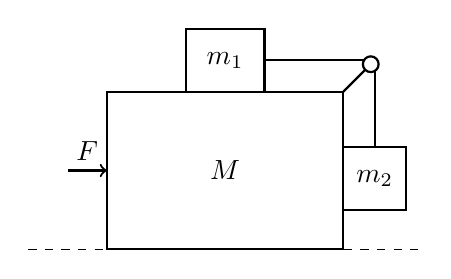
\begin{tikzpicture}
        % Draw ground line
        \draw[dashed] (-1,0) -- (4,0);
    
        % Draw the large block M
        \draw[thick] (0,0) rectangle (3,2);
        \node at (1.5,1) {$M$};
    
        % Draw the force vector F
        \draw[thick, ->] (-0.5,1) -- (0,1) node[midway, above] {$F$};
    
        % Draw the small block m1 on top of M
        \draw[thick] (1,2) rectangle (2,2.8);
        \node at (1.5,2.4) {$m_1$};
    
        % Draw the small block m2 on the right of M
        \draw[thick] (3,0.5) rectangle (3.8,1.3);
        \node at (3.4,0.9) {$m_2$};
    
        % Draw the pulley system
        \draw[thick] (2,2.4) -- (3.4,2.4) -- (3.4,1.3);
        \draw[thick] (3,2) -- (3.35,2.35);
        \draw[thick, fill=white] (3.35,2.35) circle(0.1);
    \end{tikzpicture}
    \end{center}    
    XXX
}

\sexercise{Una particella di massa \(m\) è vincolata a muoversi senza attrito all'interno di una superficie conica di angolo \(\alpha\).
Trovare le condizioni iniziali tale per cui la particella si muova di moto circolare uniforme rispetto
all'asse verticale del cono.}{
    XXX
}

\sexercise{Un blocco di massa \(m_1\) è posizionato sopra un blocco di massa \(m_2\) che si trova
a riposo su un piano liscio. Se il coefficiente di attrito tra i blocchi è \(\mu\), trovare il valore massimo della forza
orizzontale \(F\) che si può applicare a \(m_2\) affinché \(m_1\) non scivoli.}{
    XXX
}

\sexercise{Un corpo di massa \(m\), posto su un piano orizzontale scabro
(coefficiente di attrito \(\mu\)) è tirato da una forza \(\vec{F}\) formante un angolo
\(\alpha\) rispetto all'orizzontale. Il corpo si muove con velocità costante. Si determini l'angolo
per il quale l'intensità della forza è minima; ricavare inoltre il valore di quest'ultima.}{
    XXX
}

\sexercise{Due blocchi, \(A\) e \(B\), di massa rispettivamente \(m_a\) e \(m_b\), sono collegati
da una fune inestensibile e di massa trascurabile. Al blocco \(A\) che poggia su un piano inclinato
di angolo \(\alpha\) rispetto all'orizzontale, è inoltre vincolata una molla di costante
elastica \(k\) la cui altra estremità è fissata a un sostegno alla base del piano inclinato.
Il corpo \(B\) è appeso tramite una carrucola parallelamente al cateto verticale del cuneo così formato.
Trascurando gli attriti si ricavi il periodo di oscillazione dei due corpi attorno alla posizione di equilibrio.}{
    XXX
}

\pagebreak

\subsection{14 novembre}

\sexercise{Un ascensore sale con accelerazione costante
    \(A = -0.1g\); all'interno dell'ascensore si trova
    un piano inclinato, con inclinazione \(\alpha\)
    rispetto all'orizzontale e lunghezza \(l\).
    Alla sommità de piano inclinato viene posto, con velocità nulla,
    un corpo di massa \(m\) che scende scivolando lungo il piano.
    Si calcoli il modulo \(v\) della velocità relativa
    all'ascensore che il corpo possiede quando
    giunge in fondo al piano, supponendo che tra il corpo e il piano esiste attrito con coefficiente
    di attrito dinamico \(\mu_D\).}{
    Consideriamo un sistema di riferimento storto sul piano inclinato.
    Abbiamo quindi una forza apparente \(\vec{F}_A\).
    Scrivendo l'equazione di Newton e l'accelerazione otteniamo
    \[
        \begin{cases}
            m \frac{d^2x}{dt} = mg \sin\alpha + mA \sin\alpha - \mu_D R \\
            0 = -mg\cos\alpha - mA \cos\alpha + R
        \end{cases}
    \]
    dove \(R\) è la reazione vincolare.
    Dalla seconda ricaviamo
    \[
        R = m(g+A)\cos\alpha
    \]
    e quindi
    \begin{align*}
        m \frac{d^2x}{dt} &= m(g+A)\sin\alpha - \mu_D m(g+A) \cos\alpha \\
        &= m(g+A)(\sin\alpha - \mu_D\cos\alpha) \\
        &= \frac{11}{10}g(\sin\alpha - \mu_D \cos\alpha)
    \end{align*}
    Integriamo
    \[
        \frac{dx}{dt} = \frac{11}{10}g(\sin\alpha - \mu_d \cos\alpha)(t-t_0)
    \]
    e quindi
    \[
        x(t) = \frac{11}{20}g(\sin\alpha - \mu_D \cos\alpha){(t-t_0)}^2
    \]
    allora
    \[
        t-t_0 = \frac{\sqrt{x}}{\sqrt{\frac{11}{20}g(\sin\alpha - \mu_D\cos\alpha)}}
    \]
    e sostituendo nella velocità troviamo \(v(t) \rightarrow v(x)\)
    \[
        v(x) = \sqrt{
            \frac{11}{5}(\sin\alpha - \mu_D \cos\alpha)gx
        }
    \]
    e allora troviamo \(v(l)\) sostituendo \(x=l\).
}

\sexercise{Una pallina si trova ferma alla base di un piano inclinato di \(\alpha\)
rispetto all'orizzontale e di altezza \(h\), montato sopra un carrello.
Il carrello viene messo in movimento con accelerazione costante
\(A\) per un intervallo di tempo \(\tau\), dopodiché il carrello prosegue
di moto uniforme. Si determinino i valori di \(A\) per i quali la pallina, scivolando
senza attrito lungo il piano inclinato, ne raggiunge la sommità.}{
    Il moto va descritto in due fasi distinte.
    Consideriamo un sistema di riferimento storto sul piano inclinato.
    Abbiamo quindi una forza apparente \(\vec{F}_A\).
    \[
        \begin{cases}
            m\frac{d^2x}{dt^2} = -mg\sin\alpha + mA\cos\alpha & t \leq \tau \\
            m\frac{d^2x}{dt^2} = -mg\sin\alpha & t > \tau
        \end{cases}
    \]
    La velocità e la posizione al tempo \(\tau\) è data da
    \[
        v(\tau) = \tau(A\cos\alpha - g\sin\alpha)
    \]
    e
    \[
        x(\tau) = \frac{1}{2}(A\cos\alpha - g\sin\alpha)\tau^2
    \]
    Queste sono le condizioni iniziali per il secondo sistema.
    Integrando troviamo
    \[
        v(t) = v(\tau) - g\sin\alpha(t-\tau)
    \]
    e
    \[
        x(t) = x(\tau) + v(\tau)(t-\tau) - \frac{1}{2}g\sin\alpha(t-\tau)
    \]
    Troviamo il tempo \(t^*\) per cui la velocità è nulla, quindi \(v(t)=0\) cioè
    quando la pallina di ferma
    \begin{align*}
        v(\tau) - g\sin\alpha(t^* - \tau) = 0 \\
        t^* = \tau + \frac{v(\tau)}{g\sin\alpha}
    \end{align*}
    la posizione in cui la pallina si ferma è
    \begin{align*}
        x(t^*) = x^* = x(\tau) + \frac{1}{2}\frac{v^2(\tau)}{g\sin\alpha}
    \end{align*}
    Quindi la pallina raggiunge la cima se \(x^*\sin\alpha \geq h\).
    Abbiamo quindi la disequazione
    \begin{align*}
        \frac{1}{2}(A\cos\alpha - g\sin\alpha)\tau^2\sin\alpha + \frac{{(A\cos\alpha  - g\sin\alpha)}^2\tau^2}{2g} \geq h
    \end{align*}
    che ha soluzioni
    \[
        A \geq
        \frac{g\sin\alpha + \sqrt{g^2\sin^2\alpha + \frac{8hg}{\tau^2}}}{2\cos\alpha}
    \]
}

\sexample{Un tubicino cilindrico rigido, di sezione trascurabile, ruota in un piano
verticale, con velocità angoalre costante \(\omega\) intorno a un asse orizzontale;
dentro il tubicino può sciovlare senza attrito una pallina di massa \(m\). All'istante \(t=0\)
il tubicino è in posizione verticale, la pallina si trova al di sopra dell'asse di rotazione,  a distanza \(d\)
da esso e con velocità nulla rispetto al tubicino. Si studi il motivo della pallina lungo il tubicini,
approssimando la pallina a un punto materiale. Si discuta la soluzione nel caso
\(\omega \to 0\) e \(\omega \gg 1\).}{
    Scegliamo un sistema di riferimento con gli assi solidali al cilindro (\(x\) è la direzione verticale del cilindro).
    Sulla pallina agisce la forza peso, la reazione vincolare
    e la forza apparente (la forza centrifuga verso l'esterno e la forza di Coriolis).
    La reazione vincolare punta sull'asse delle \(y\).
    Abbiamo quindi
    \[
        \vec{F}_{CE} = -m \vec{\omega} \wedge (\vec{\omega} \wedge \vec{r})
    \]
    e
    \[
        \vec{F}_{CO} = -2m \vec{\omega} \wedge \vec{v}
    \]
    Allora
    \begin{align*}
        \vec{F}_{CE} &= -m \omega^2 \wedge \hat{z} \wedge (\hat{z} \wedge{x}) \\
        &= m\omega^2 \wedge \hat{x}
    \end{align*}
    e
    \begin{align*}
        \vec{F}_{CO} &= -2m\omega \frac{dx}{dt} (\hat{z} \wedge \hat{x}) \\
        &= 2m\omega \frac{dx}{dt} \hat{y}
    \end{align*}
    Adesso possiamo scrivere le equazioni di Newton
    \[
        \begin{cases}
            m\frac{d^2 x}{dt} = -mg\cos\theta + m\omega^2 x \\
            m\frac{d^2 y}{dt} = -mg\sin\theta + 2m\omega \frac{dx}{dt} + R = 0
        \end{cases}
    \]
    La massa si semplifica risultando nell'equazione non omogenea
    \[
        \frac{d^2x}{dt} - \omega^2 x = -g\cos(\omega t)
    \]
    La soluzione è data dalla combinazione lineare
    di una soluzione particolare dell'equazione omogenea. Quindi
    \[
        x(t) = Ae^{\omega t} + Be^{-\omega t} + \frac{g}{2\omega^2}\cos(\omega t)
    \]
    con le condizioni iniziali troviamo
    \[
        x(t) = \left(d-\frac{g}{2\omega^2}\right)
        \cosh(\omega t) + \frac{g}{2\omega^2}\cos(\omega t)
    \]
    dove \(d\) è la lunghezza del tubo da dove parte la pallina.
    Studiamo ora il limite \(\omega \to 0\).
    Notiamo gli asintotici
    \[
        \cos(\omega t) \sim 1 - \frac{\omega^2 t^2}{2}
    \] e
    \[
        \cosh(\omega t) \sim 1 + \frac{\omega^2 t^2}{2}
    \]
    (gli asintotici possono essere usati con la somma se i termini più grandi che consideriamo non si semplificano).
    Allora
    \begin{align*}
        x(t) &\sim \left(d - \frac{g}{2\omega^2}\right)
        \left(1 + \frac{\omega^2t^2}{2}\right)
        + \frac{g}{2\omega^2}\left(1 - \frac{\omega^2t^2}{2}\right) \\
        &= d - \frac{g}{2}t^2
    \end{align*}
    Quindi, se la velocità è molto bassa, la forza di gravità domina.
    Se \(\omega \gg 1/t\) abbiamo
    \begin{align*}
        x(t) \sim \frac{1}{2}de^{\omega t}
    \end{align*}
    Quindi se \(\omega\) è grande domina la forza centrifuga e la pallina viene sparata fuori.
}

% Integral command
\ExplSyntaxOn
\DeclareDocumentCommand{\integral}{d[] d[] d[] d[]}
{
    \IfNoValueTF { #4 }
    {
        \IfNoValueTF { #3 }
        { \int #1\,d#2 }
        { \text{Either\,\,2\,\,or\,\,4\,\,arguments\,\,must\,\,be\,\,passed} }
    }
    {
        \int\limits\c_math_subscript_token{#1}^{#2} #3 \,d#4
        % In Expl Syntax characters as '_' or ':' are used as letters in command names
        % hence the \c_math_subscript_token{#1} rather than _{#1}
    }
}
\ExplSyntaxOff

\sexercise{Si supponga che una goccia di pioggia cadendo attraverso una nuvola accumuli massa ad un rate \(kmv\),
dove \(k > 0\) è una costante, \(m\) è la massa della goccia e \(v\) la sua velocità.
Si trovi la velocità della goccia a un generico tempo \(t\)
supponendo che parta a riposo, trovare inoltre la massa della goccia allo stesso tempo.}{
    Abbiamo che
    \[
        \frac{dm}{dt} = kmv
    \]
    e 
    \begin{align*}
        m(t)g &= \frac{d}{dt}\left(m(t)v(t)\right) \\
        &= m(t)\frac{dv(t)}{dt} + v\frac{dm(t)}{dt}
    \end{align*}
    Allora troviamo l'equazione differenziale
    \begin{align*}
        m(t)g &= m(t) \frac{dv}{dt} + km(t)v^2 \\
        g &= \frac{dv}{dt} + kv^2
    \end{align*}
    che si risolve integrando
    \begin{align*}
        \integral[0][v][\frac{1}{g-kv^2}][v]
        = \integral[0][t][][t]
    \end{align*}
    da cui troviamo
    \[
        v(t)= \sqrt{\frac{g}{k}} \tanh(\sqrt{kg}t)
    \]
    Per trovare la massa
    \[
        \integral[m_0][m][\frac{1}{m}][m]
        = \integral[0][t][\sqrt{kg}\tanh(\sqrt{kg}t)][t]
        = m_0 \cosh(\sqrt{kg}t)
    \]
}

\sexercise{Un punto materiale di massa \(m\) è appeso tramite una molla di costante
    elastica \(k\) ad un supporto che avanza con accelerazione \(a\).
    Clcolare l'allungamento della molla.}{
    
}

\sexercise{Un piano inclinato 3-4-5 è fissato su una piattaforma rotante. Un blocco è posizionato
    a riposo sul piano e il coefficiente d'attrito statico fra il blocco e il piano è
    \(\mu_s\). Il blocco è inizialmente alla distanza di \(40\) cm dal centro della piattaforma.
    Trovare il valore minimo della velocità angolare \(\omega\) che impedisce al blocco di cadere 
    sulla piattaforma.}{
    XXX
}
\begin{figure*}[h]
    \begin{center}
        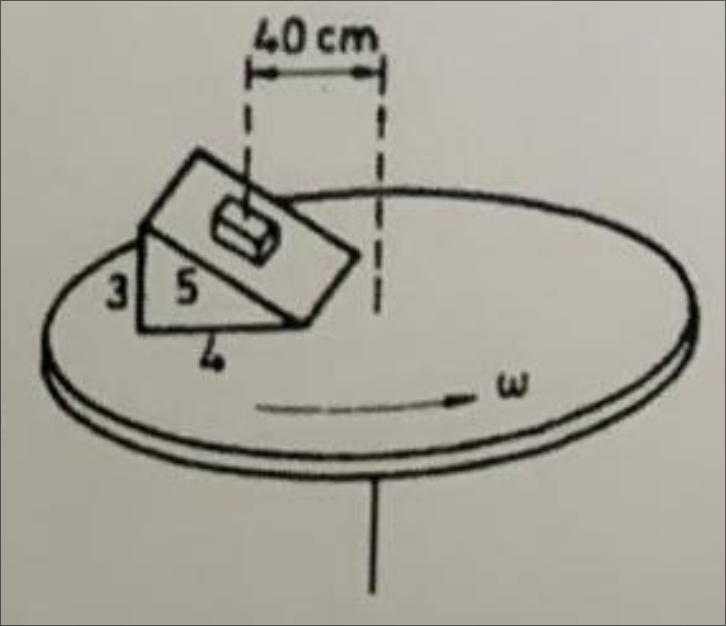
\includegraphics[width=.5\textwidth]{media/es_5_6.png}
    \end{center}
\end{figure*}

\end{document}